\chapter{Systemdesign}\label{Systemdesign}
Der er udarbejdet forskellige diagrammer på baggrund af de specificerede systemkrav.  Diagrammerne har til formål at dele systemet op i realiserbare dele for at vise designet af systemet. 

\section{Pakkediagram}
Pakkediagrammet figur \ref{Pakkediagram} giver en oversigt over afhængighederne i PC Applikation.
For at slippe for cykliske forbindelser blev mange datastrukturer flyttet fra CalculationLibrary, ComputerVisionLibrary og RoboLibrary til DataStructures-biblioteket.
DataStructures indeholder altså kun nogle datastrukturer og nogle extension-metoder til disse. 
For forklaringen af indholdet af de øvrige pakker, se klassediagrammerne for hvert bibliotek.

AutoSocograophyWPF inderholder alt, der hører til Grafisk brugergrænseflade (GUI), herunder de tre menuer, 3DscanMenu, StartMenu og UltrasoundMenu. 

ComputerVisionLibrary indeholder klasser, der har at gøre med 3D billedet og konvetering til et mesh, herunder ComputerVisionMaster, KinectsFusionizer og PLYExporter. 

RoboLibray pakken indeholder klasser som robotarmen skal benytte for at kunne flytte sig, herunder Analyzer, Data, Logic, Modbus, PathCreator, PathFeeder, Reader, RoboMaster, URPose og Writer. 

DataStructures

CalculationLibrary

\begin{figure}[H]
    \centering
    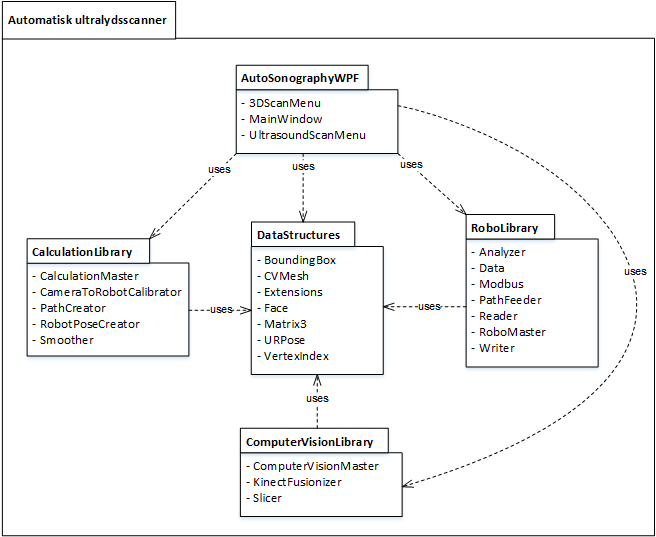
\includegraphics[width=1\textwidth]{figurer/d/Design/Pakkediagram}
    \caption{Pakkediagram for Automatisk Ultralydsscanner}
    \label{Pakkediagram}
\end{figure}
\newpage

\section{Klassediagram}
Dette afsnit beskriver klasserne fra pakkediagrammet. Klassediagrammerne viser strukturen i systemet og deres relationer. Hver klasse indeholder de vigtigste metoder og attributer i klassen, der udgør funktionaliteten i PC Applikation. 

\subsection{GUI}
Denne klasse indeholder brugergrænsefladen af PC Applikation.

\let\labelitemi\labelitemii
\begin{itemize}
\item{MainWindow}\newline
Giver anledning til at foretage et 3D scan. Såfremt en 3D scanning er gennemført giver det også anledning til at starte en ultralydsscanning.
Når menuen startes, oprettes en instans af RoboMaster, for at sætte Robotarm i standard positur. Dette er nødvendigt, hvis Robotarm skulle være i vejen for en 3D scanning.
Hvis der ikke er nogen forbindelse til Robotarm vil der 

\item{3DScanMenu}\newline
I denne menu er der mulighed for at se det nuværende dybdebillede, afgrænse området der skal 3D scannes og foretage en 3D scanning.

\item{UltrasoundScanMenu}\newline
I denne menu kan den procentvise færdiggørelse af ultralydsscanningen følges. Der er også mulighed for at pause samt afbryde ultralydsscanningsprocessen.
\end{itemize}

\begin{figure}[H]
    \centering
    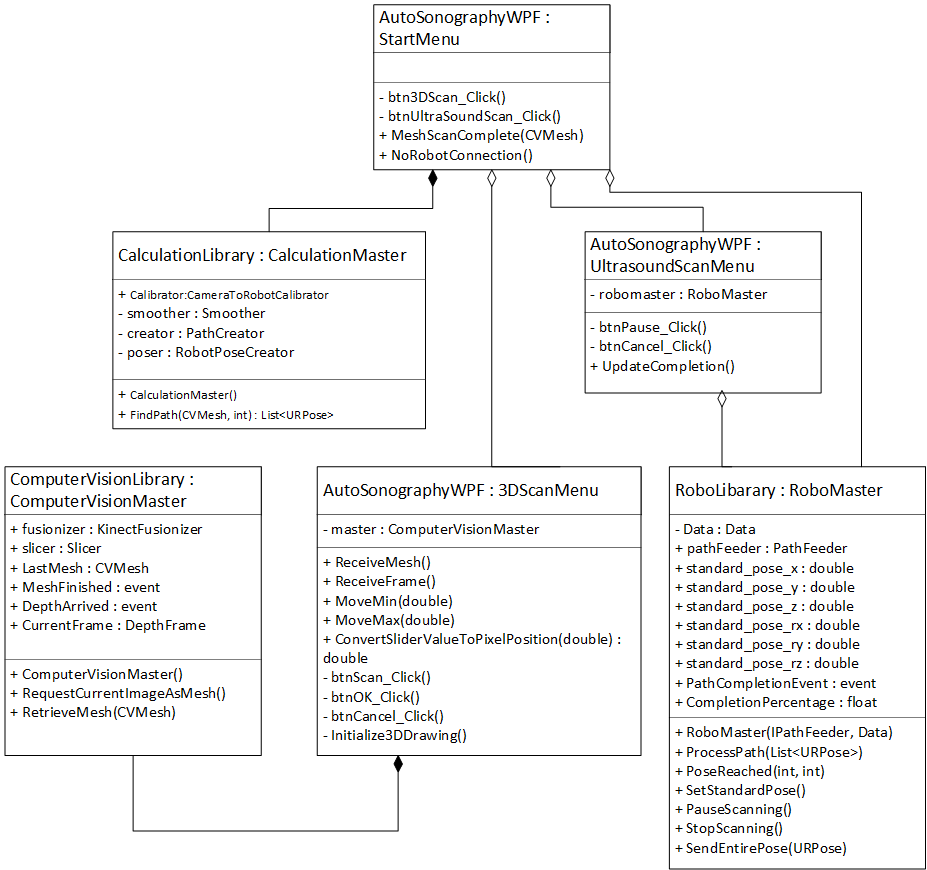
\includegraphics[width=1\textwidth]{figurer/d/Design/Class/uml_class_gui}
    \caption{Klassediagram for GUI}
    \label{class_gui}
\end{figure}
\newpage

\subsection{ComputerVisionLibrary}
Formålet med dette bibliotek er at få en afgrænset 3D scanning fra et 3D kamera.

\begin{itemize}
\item{KinectFusionizeren}\newline
Har til ansvar at åbne Kinect-sensoren, tage det nuværende dybdebillede fra sensoren og konvertere det til en mesh.

\item{ComputerVisionMaster}\newline
Denne klasse virker som den logiske grænseflade til KinectFusionizeren, hvor instansen af den nuværende mesh lagres her.
Andre klasser kan subscribe til ComputerVisionMasteren for at høre hvornår der er en ny mesh tilgængelig.

\item{Slicer}\newline
Denne klasse sørger for at fjerne de punkter i en mesh der er uinteressante:
\begin{enumerate}
\item{Faces der peger nedaf, dvs fejlpunkter. Da 3D kameraet er monteret i loftet, vil den ikke kunne se undersiden af det den skanner.}
\item{Duplikerede punkter. KinectFusionizer outputter punkter der er ens. Disse fjernes af optimeringsårsager.}
\item{Punkter og faces der er uden for det område der ønskes skannet. Dette inkluderer nærtliggende objekter som fx en væg, eller områder på patienten der ikke ønskes skannet.}
\end{enumerate}
\end{itemize}

\begin{figure}[H]
    \centering
    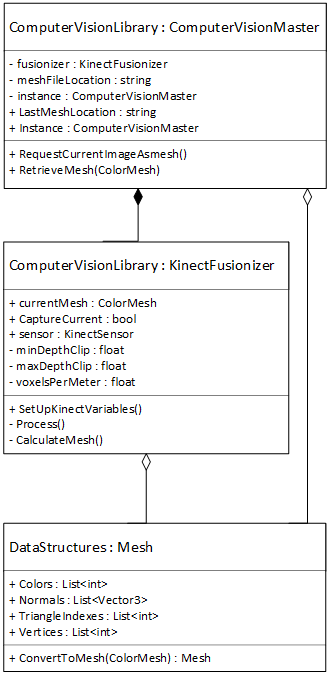
\includegraphics[width=1\textwidth]{figurer/d/Design/Class/uml_class_computervisionlibrary}
    \caption{KLassediagram for ComputerVisionLibrary}
    \label{class_ComputerVisionLib}
\end{figure}
\newpage

\subsection{CalculationLibrary}
Dette bibliotek agerer som bindeledet mellem ComputerVisionLibrary og RoboLibrary.

\begin{itemize}
\item{CameraToRobotCalibrator} \newline
Sørger for at konvertere 3D scanningen givet fra ComputerVisionLibrary fra 3D Kameras rum til Robot Arms rum.
Dette sker ved en kæde af matrix-transformationer i en speciel rækkefølge. 
Normaltvis har man en translation, rotation og skalering, men da Robot Arms og 3D Kameras koordinatsystemer begge er angivet i millimeter, er skaleringen unødvendig.
I tilfældet for dette projekt sker der først en rotering og derefter en translation, for at bestemme transformationsmatricen. 
Hvert punkt i en mesh konverteres så til det nye space.

\item{Smoother}\newline
Denne klasse har til ansvar at udjævne en mesh. Med udjævning forstås at 'ensforme' normalerne, altså retningsvektorer i en mesh's faces.
Dette er nødvendigt da 3D Kameras output kan være uperfekt og dermed vil normalerne være ekstreme/deforme. Udjævningen sker gennem laplacian smoothing, se \cite{Smooth} for forklaring af algoritme.

\item{PathCreator}\newline
Klassen afgør listen af punkter i en mesh som der skal findes positurer til Robot Arm ud fra.
For at afgøre stien genereres der en 'bølge' - i implementeringen en squarewave - af punkter der draves over meshen.
De vertices i meshen der tilnærmer sig punkterne i bølgen bedst vil blive udvalgt til stien.

\item{RobotPoseCreator}\newline
I denne klasse vil konverteringen af en mesh-sti til en liste af positurer ske.
For hvert punkt i mesh-stien, vil en vertex' normal findes. 
Ved hjælp af normalen, sti-punktets koordinater samt længden på Robotarms probe kan den forskudte Robot Arm position findes.
Inverteres denne normal, kan det ses som en retningsvektor for en Robotarm.
Retningsvektoren konverteres først til en roll, pitch og yaw - altså roteringer omkring de tre retningsakser; X, Y og Z.
Da man ikke kan afgøre alle tre værdier ud fra en retningsvektor alene, sættes pitch til 0. Disse værdier konverteres herefter til en rotationsvektor.
Positionsvektoren og rotationsvektoren udgør til sammen en positur, som tilføjes til listen af positurer.
\end{itemize}

\begin{figure}[H]
    \centering
    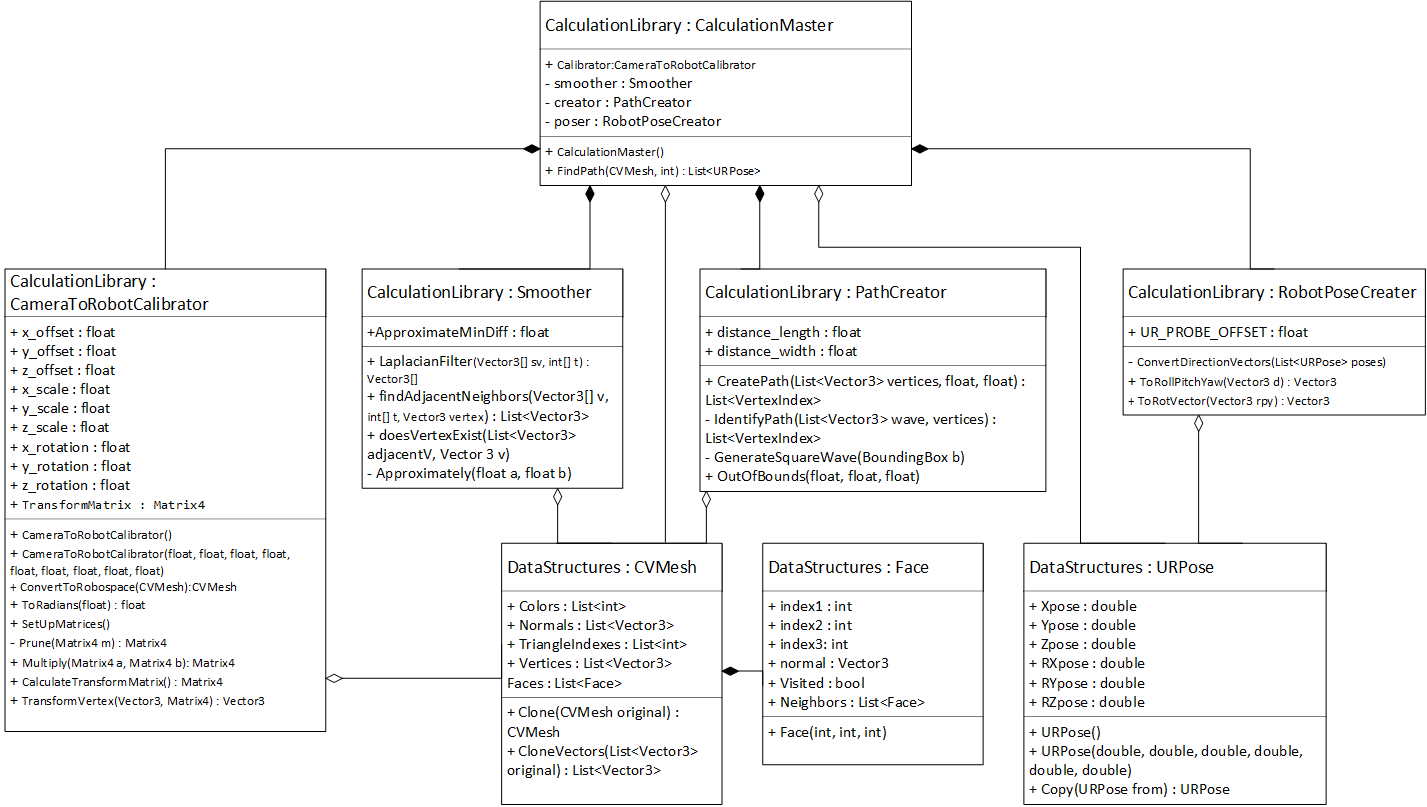
\includegraphics[width=1\textwidth]{figurer/d/Design/Class/uml_class_calculationlibrary}
    \caption{KLassediagram for CalculationLibrary}
    \label{class_ConversionLib}
\end{figure}
\newpage

\subsection{RoboLibrary}
Biblioteket giver mulighed for kommunikation med Robot Arm.

\begin{itemize}
\item{RoboMaster}\newline
Klassen agerer som bindeled mellem de øvrige klasser i biblioteket og GUI.

\item{PathFeeder} \newline
Står for at gennemløbe hver positur i listen, og kommunikere med Data for at finde ud af hvornår den næste positur skal sendes til Robot Arm.

\item{Data}\newline
Klassen virker som en grænseflade mellem den 'logiske' del af biblioteket og dens underliggende reader/writer klasser.

\item{Reader}\newline
Denne klasse står for kontinuerligt at læse data fra Robot Arm, for at afgøre dens nuværende positur. 

\item{Analyzer} \newline
Klassen konverterer det indlæste data til en objekt-orienteret model, altså transformation af bytes til Robot Arms nuværende positur.

\item{Writer}\newline
Klassen har til ansvar at omskrive værdier til binær data. Den omskriver både positurer samt konfigurationer.

\item{Modbus}\newline
Denne klasse skriver binær data ud på Robot Arms IP gennem modbus-protokollen.
\end{itemize}

\begin{figure}[H]
    \centering
    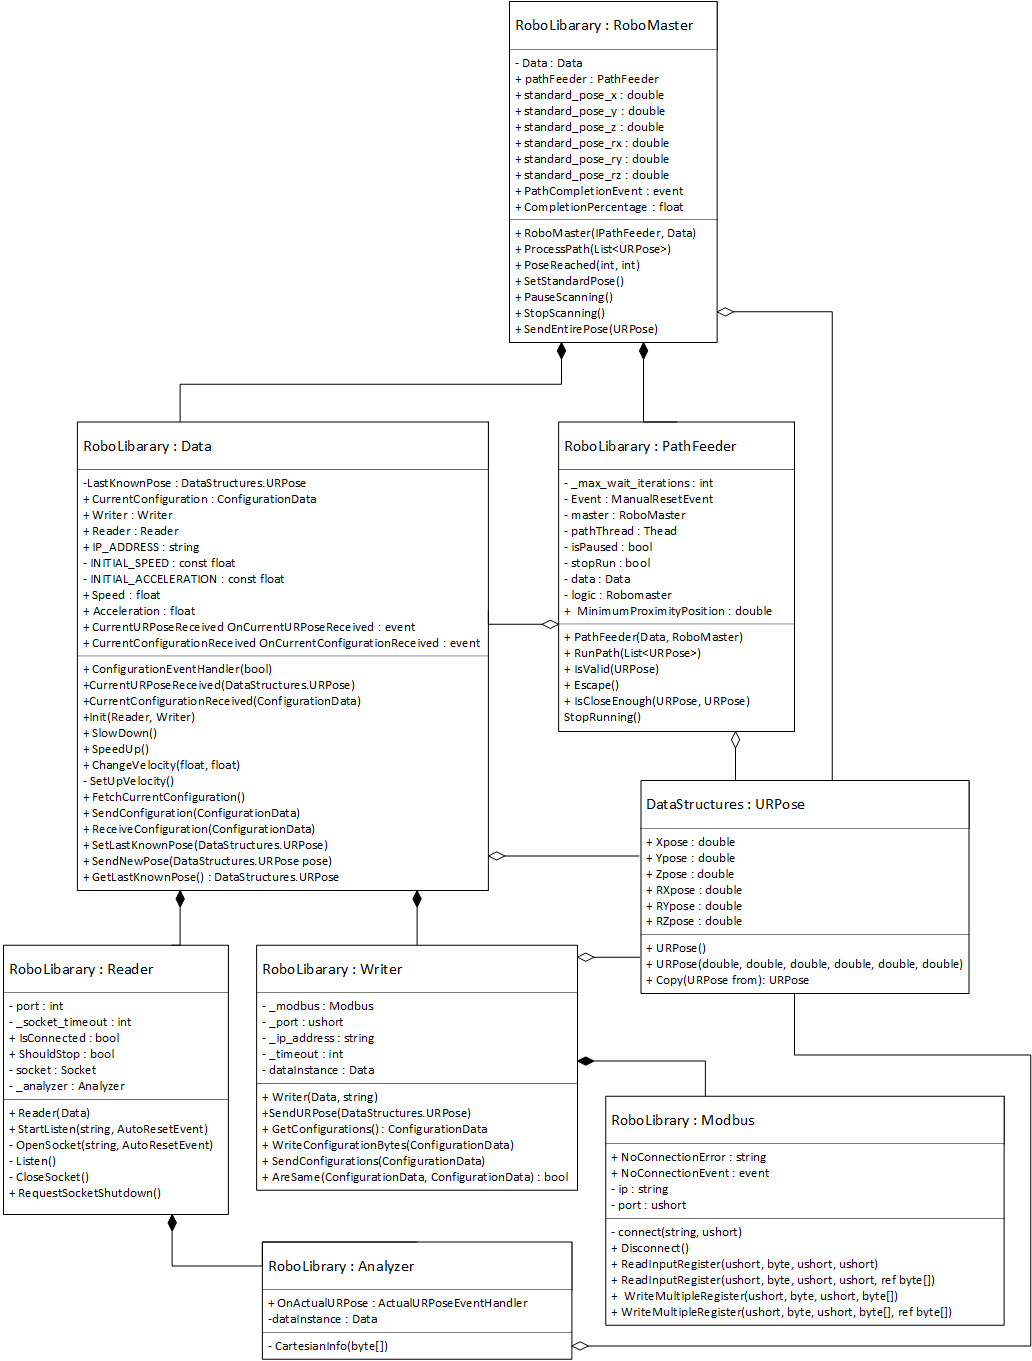
\includegraphics[width=1\textwidth]{figurer/d/Design/Class/uml_class_robolibrary}
    \caption{KLassediagram for RoboLibrary}
    \label{class_RoboLib}
\end{figure}

\newpage
\section{Sekvensdiagrammer}
Der er på baggrund af klassediagrammerne lavet sekvensdiagrammer, som beskriver systemets funktionalitet, og hvor de vigtigse metoder og attributter imellem klasserne er identificeret.

Nedenstående sektioner vil beskrive de vigtigste sekvensdiagrammer i system og fremvise, hvordan klasserne indbyrdes kommunikerer. 

\subsection{Read Robot Data} 
Reader initieres med en IP hvor den skal lytte på. 
Der åbnes en socket på denne IP, og derefter lytter den kontinuert i en baggrundstråd. 
Readeren giver de rå data videre til Analyzer som konverterer dem til Robot Arms nuværende positur.

\begin{figure}[H]
    \centering
    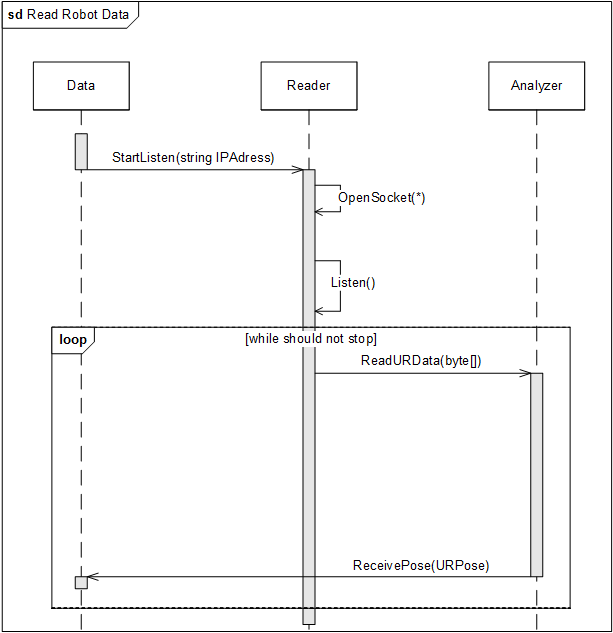
\includegraphics[width=1\textwidth]{figurer/d/Design/Sequence/sd_reading}
    \caption{Sekvensdiagram for Read Robot Data - indlæsning af Robotarms positur}
    \label{sd_reading}
\end{figure}

\subsection{3D scan}
Ved scan vil KinectFusionizeren stå for at tage et dybdebillede fra Kinect-sensoren.
Den vil dernæst konvertere dybdebilledet til en point cloud.Dette trianguleres, så der fås en mesh der efterfølgende kan bearbejdes. 3DScanMenu modtager meshen gennem event-kommunikation.
Gennem de beskræringsparametre der er valgt i menuen vil meshen dernæst beskæres i Slicer, så kun det ønskede område fremkommer. Efter beskæringen vises meshen som en rotérbar 3D model i menuen.

\begin{figure}[H]
    \centering
    \includegraphics[width=1\textwidth]{figurer/d/Design/Sequence/sd_3Dscan}
    \caption{Sekvensdiagram for 3D scan}
    \label{sd_3Dscan}
\end{figure}
\newpage

\subsection{Feed Path}
Efter konvertering af mesh output til robot positur sti, vil listen af positurer sendes fra RoboMaster til PathFeeder. 
Se sekvensdiagrammet 'Path Creation' for en gennemgang af hvordan disse positurer findes.
PathFeeder gennemløber hver positur og sender den næste i listen til Data, som videregiver posituren til Writer.
RoboMaster informeres løbende om hvor langt PathFeeder er med at gennemløbe punkter.
Writer konverterer posituren til binær data, og ModBus skriver dataen ud på Robot Arms register.
Hernæst ser PathFeeder på om Robot Arms nuværende positur har nærmet sig den ønskede positur. 
Når den er tæt nok på, hoppes der ud af 'while'-løkken, og den næste positur kan sendes.
Den Alt der er her skal forstås som at PathFeeder kører i sin egen baggrundstråd der kan pauses. 
Ved terminering af denne baggrundstråd vil PathFeeder stoppe med at videregive nye positurer til Robot Arm.

\begin{figure}[H]
    \centering
    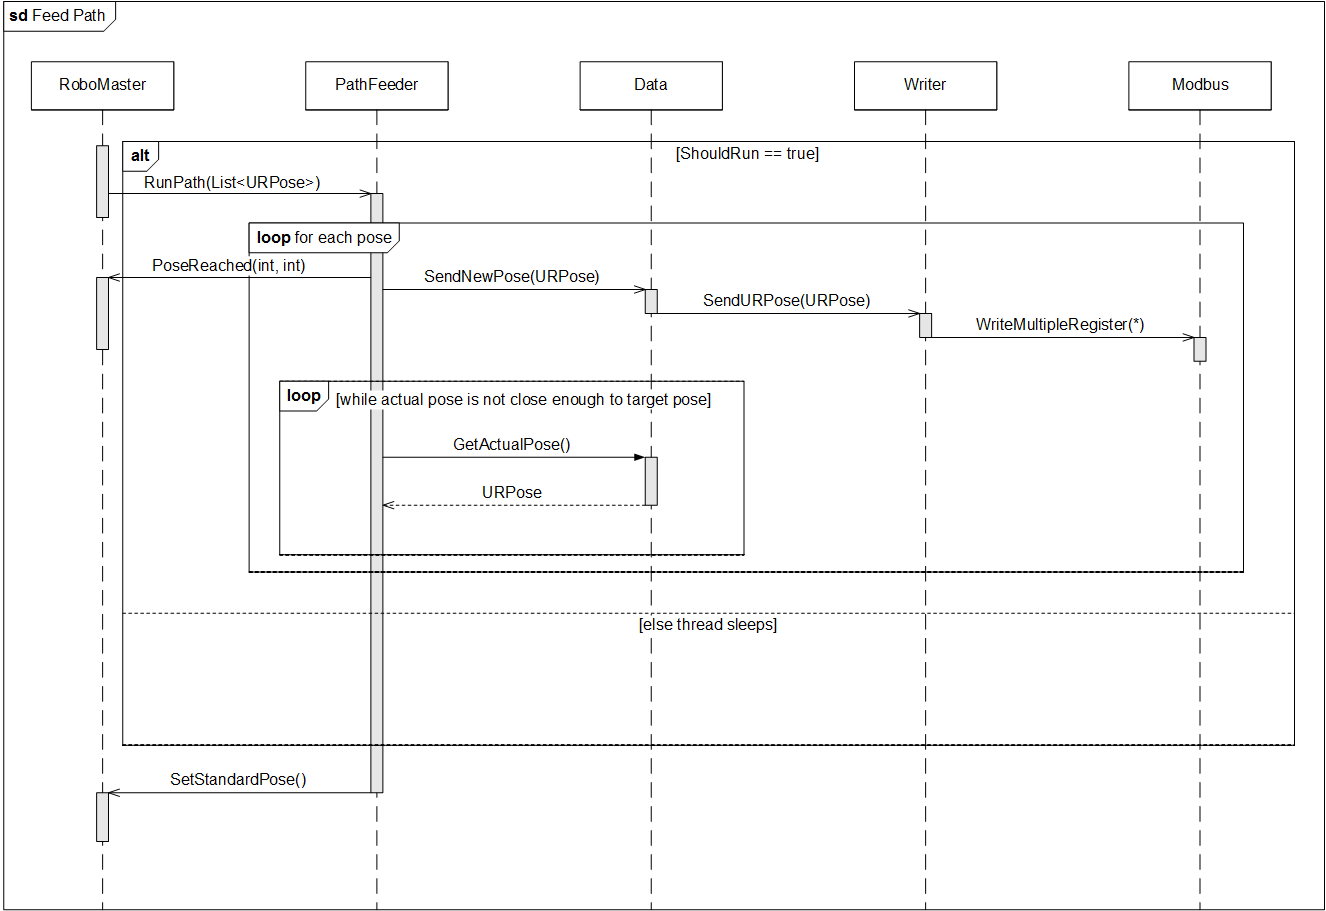
\includegraphics[width=1\textwidth]{figurer/d/Design/Sequence/sd_feedpath}
    \caption{Sekvensdiagram for Feed Path}
    \label{sd_feedpath}
\end{figure}

\subsection{Pathcreation}
Ved tryk på Ultralydsscan-knappen sendes den scannede mesh videre til CalculationMaster. Se sekvensdiagrammet '3D scan' for at se hvordan den scannede mesh opnås.
Først skal meshen konverteres fra 3D Kameras rum til Robot Arms rum, dette sker i CameraToRobotCalibrator, hvor meshen roteres og translateres ift. hvor 3D Kamera befinder sig i virkeligheden.
Efter transformationen skal meshen udjævnes, så de rå og ekstreme normaler i meshen udglattes. Loopet afgør hvor mange gangen meshen skal gennemkøres filteret.
Dernæst sendes den konverterede mesh til PathCreator så der oprettes en liste af de punkter i meshen vi ønsker at Robot Arm skal gennemgå.
Til sidst skal stien der findes i PathCreator konverteres til Robot Arm positurer, da stien i PathCreator kun fortæller position direkte på meshen.
Med denne sti får Robot Arm afdækket overfladen på Patient, hvis den har en Ultralydsscanner monteret.
Stien kan nu videresendes til RoboMaster - se sekvensdiagrammet 'Feed Path' Figur \ref{sd_feedpath}.

\begin{figure}[H]
    \centering
    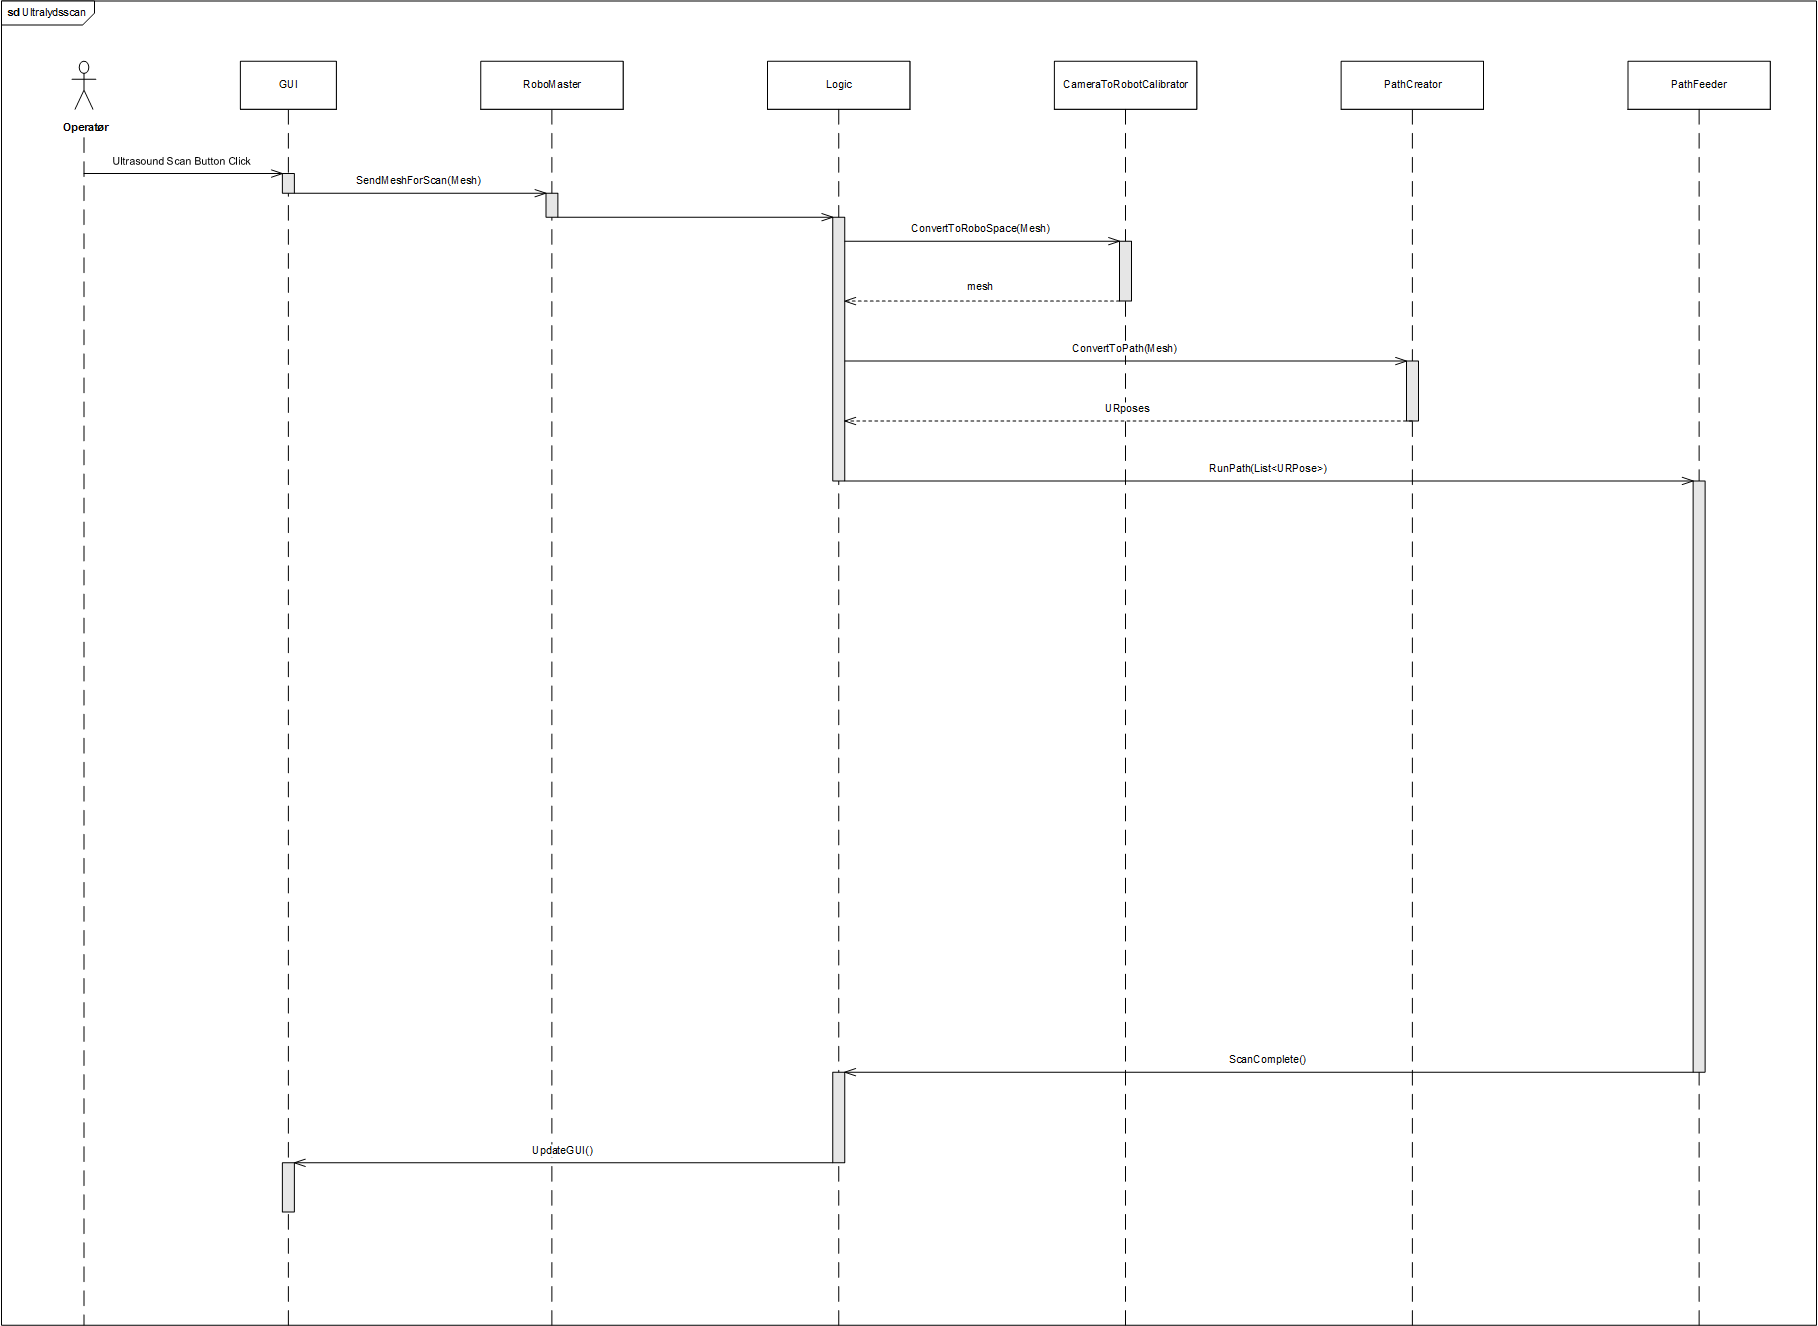
\includegraphics[width=1.4\textwidth, angle =90]{figurer/d/Design/Sequence/sd_ultrascan}
    \caption{Sekvensdiagram for Pathcreation}
    \label{sd_ultrascan}
\end{figure}
\newpage

\section{Detajleret specifikation af klassediagrammer}
Her skal der vises metoderne i hver klasse. 

\section{Tilstandsdiagram}
Dette afsnit beskriver adfærden i systemet ved brug af et tilstandsdiagram. Tilstandsdiagrammet beskriver overgange mellem forskellige tilstande. I UC3: Ultralydsscan brystområde kan Operatør vælge at pause scanningen midlertidig og enten genoptage eller helt stoppe scanning. Figur \ref{stm_Ultra} beskriver Robotarms forskellige tilstande under udførelse af ultralydsscanning. 

\begin{figure}[H]
    \centering
    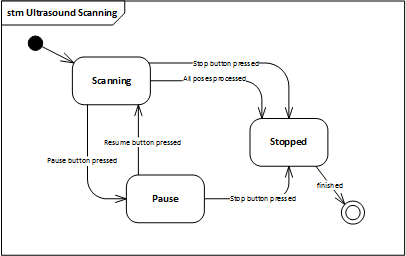
\includegraphics[width=0.7\textwidth]{figurer/d/Design/stm_UC3}
    \caption{Tilstandsdiagram for ultralydsscanning}
    \label{stm_Ultra}
\end{figure}

\section{Beregninger} 
Bare for at have det et sted og forsøge 

%% Laver piecewise funktionen 
\[ roll = \begin{cases} 
      \frac{\pi}{2}-sin^{-1}(z) & y\leq 0 \\
      \pi +cos^{-1}(-z) & y > 0 \\
   \end{cases}
\]



$$ pitch = -(\pi -atan2(y,x)) $$ Er vel det samme som   $$ pitch = atan2(y,x) - \pi $$


\[yaw = 0\] 

%%%%%%%%%%%%%%%%%%%%
% Matricerne 
\[R_M = \begin{bmatrix}
    1 & 0 & 0 \\
    0 & cos(roll) & -sin(roll) \\
    0 & sin(roll) & cos(roll)
\end{bmatrix}\] 


\[P_M = \begin{bmatrix}
    cos(pitch) & 0 & sin(pitch) \\
    0 & 1 & 0 \\
    -sin(pitch) & 0 & cos(pitch)
\end{bmatrix}\] 


\[Y_M = \begin{bmatrix}
    cos(yaw) & -sin(yaw) & 0 \\
    sin(yaw) & cos(yaw) & 0 \\
    0 & 0 & 1
\end{bmatrix}\] 

%%%%%%%%%%%%%%%%%%%%%%%%%%%% 
\[roll \geq (-\pi,\pi) \]
\[pitch \geq (-\pi,\pi) \]


\[\mathbb{R} = Y_M \cdot P_M \cdot R_M \]

%%%%%%%%%%%%%%%%%%%%%%%%
% Definerer alpha 
\[\alpha = cos^-1\bigg(\frac{\mathbb{R}_{0,0}+\mathbb{R}_{1,1}+\mathbb{R}_{2,2}-1}{2}\bigg)\] 


%%%%%%%%%%%%%%%%%%%%%% 
%Theta er lig med beregnes her 

\[ \theta = \begin{cases} 
      \alpha &  roll\geq 0 \land pitch \geq 0  \\
      2\pi-\alpha  &  roll < 0 \lor pitch < 0 \\
   \end{cases}
\]

%%%%%%%%%%%%%%%%%%%%%%% 

% mu beregnes her 
\[\mu = \frac{1}{2*sin(\theta}\]


%%%%%%%%%%%%%%%%%%%%%% 
% r_x, r_y, r_z beregnes her 

\[r_x =\mu \times(\mathbb{R}_{2,1}-\mathbb{R}_{1,2}) \times\theta \]
\[r_y =\mu \times(\mathbb{R}_{0,2}-\mathbb{R}_{2,0}) \times\theta \]
\[r_z =\mu \times(\mathbb{R}_{1,0}-\mathbb{R}_{0,1}) \times\theta \]



